\chapter{DHCP Configuration}

\section{Background}
\paragraph{}
Every machine, from computers to servers, requires an IP address
for it to be able to send and receive packets of data or information. (\cite{masterWS19})
These IP addresses act like home addresses on a street, and whilst DNS is 
responsible for resolving those IP addresses into names, there are two ways 
of assigning IP addresses to machines. These methods are static addressing
and DHCP (\cite{masterWS19}).

\paragraph{}
Static Addressing is the process of configuring IP addresses on a system
manually. It is a hands-on approach where IP addresses
are physically plugged into the NIC settings on a particular device (\cite{masterWS19}).
Despite its simplicity, this method is not scalable in environments that host
multiple devices like a small or large company, where there are laptops, desktops, 
printers, servers or other types of machines (\cite{masterWS19}). Each of these
devices needs an IP address, however manually assign them becomes tedious at a larger scale. The solution
to this problem lies in the Dynamic Host Configuration Protocol (DHCP) (\cite{masterWS19}).

\paragraph{}
DHCP is a protocol that solves the problem of providing IP addresses for many devices
on a wide scale. It allows for machines or devices that are plugged into the network and obtain 
IP address information (\cite{masterWS19}). This ability to assign IP address information to devices 
allows for DHCP to have multiple applications. When a laptop or phone is connected to a Wi-Fi router
to gain internet access, a DHCP server allows for that device to route traffic on the network by assigning
IP addressing information (\cite{masterWS19}). When a device connects to public Wi-Fi, its DHCP server runs on the router itself
and in businesses where Windows Server serves as a datacenter, DHCP services are most often hosted 
on one or more servers across the network (\cite{masterWS19}).

\section{Configuration Steps}
\subsection{DHCP Post-Install configuration}
Like other roles, the DHCP server needs to be provided a role during the 
installation phase. After the DHCP role has been added to the server, 
it isn't yet properly configured. 

\paragraph{}
The DHCP server can give clients two kinds of access groups: DHCP Administrators and DHCP Users (\cite{DHCPgroups}).
DHCP Users have read-only access to the server, which allows them to view, but not to modify server data, including DHCP server 
configuration, registry keys, DHCP log files, and the database (\cite{DHCPgroups}). They cannot create scopes, modify options values, create 
reservations or exclusion ranges, and more.
DHCP Administrators are able to view and modify data at the DHCP server (\cite{DHCPgroups}). They can 
create and delete scopes, add reservations, change option values, create superscopes or perform
 any other activity needed to adminster the DHCP server (\cite{DHCPgroups}). Despite this overseering control, they do not 
have unlimited administrative rights,because they on have rights on the local computer only (\cite{DHCPgroups}). 

\paragraph{}
These two groups are local to the server as well, meaning they cannot authorize DHCP Servers. 
This can only be done by Domain Admins(\cite{DHCPgroups}). Authorizing the server is needed because DHCP communication typically occurs before any user
or computer authentiation. DHCP protocols are based on IP protocols as well, therefore, an unknown DHCP server could 
provide invalid information to clients. Authorization prevents this (\cite{DHCPauthor}).

\paragraph{}
The authorization of the DHCP server in the wizard required for users to be 
given credentials that they would need to access the server on a user level. So far the only 
credential set was \texttt{OPS\textbackslash{}Administrator}.For any users who attempt to 
connect to the server in future, they must use this username. 

\begin{figure}[H]
    \centering
    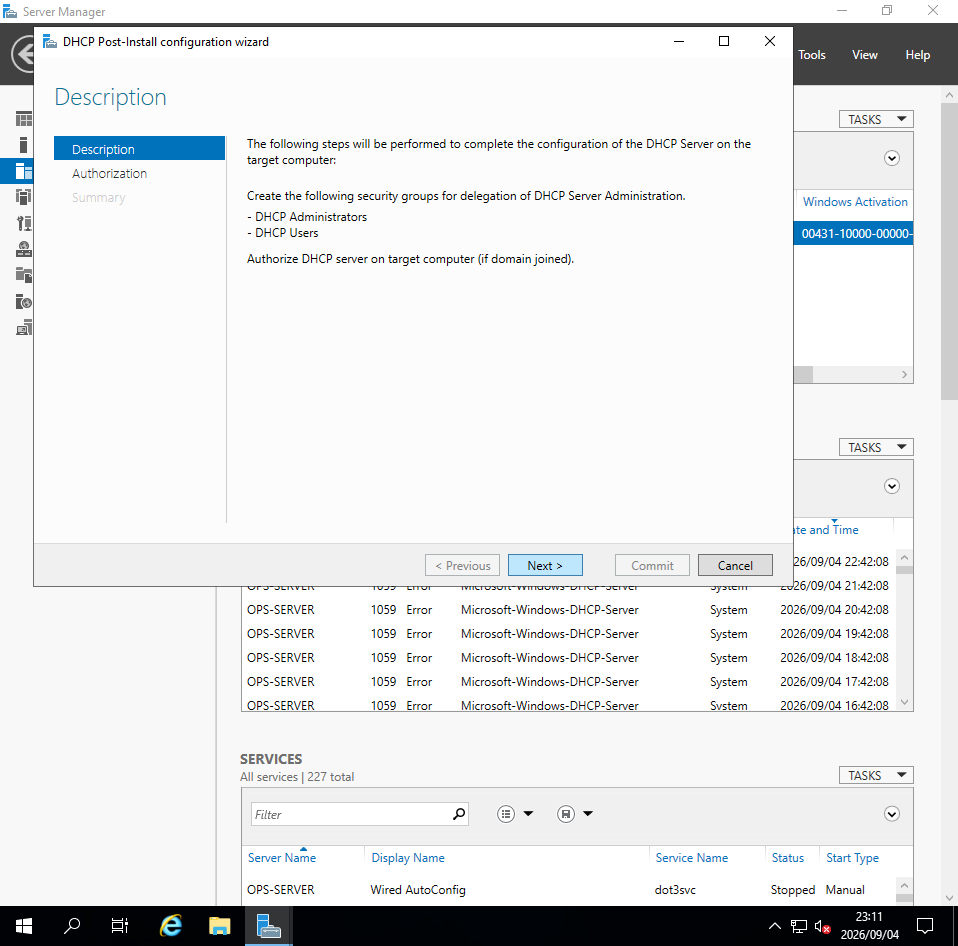
\includegraphics[width=0.7\linewidth]{Images/DHCP/DHCP_01.png}
    \caption{Description of DHCP Post-Install Configuration Wizard}
\end{figure}

\begin{figure}[H]
    \centering
    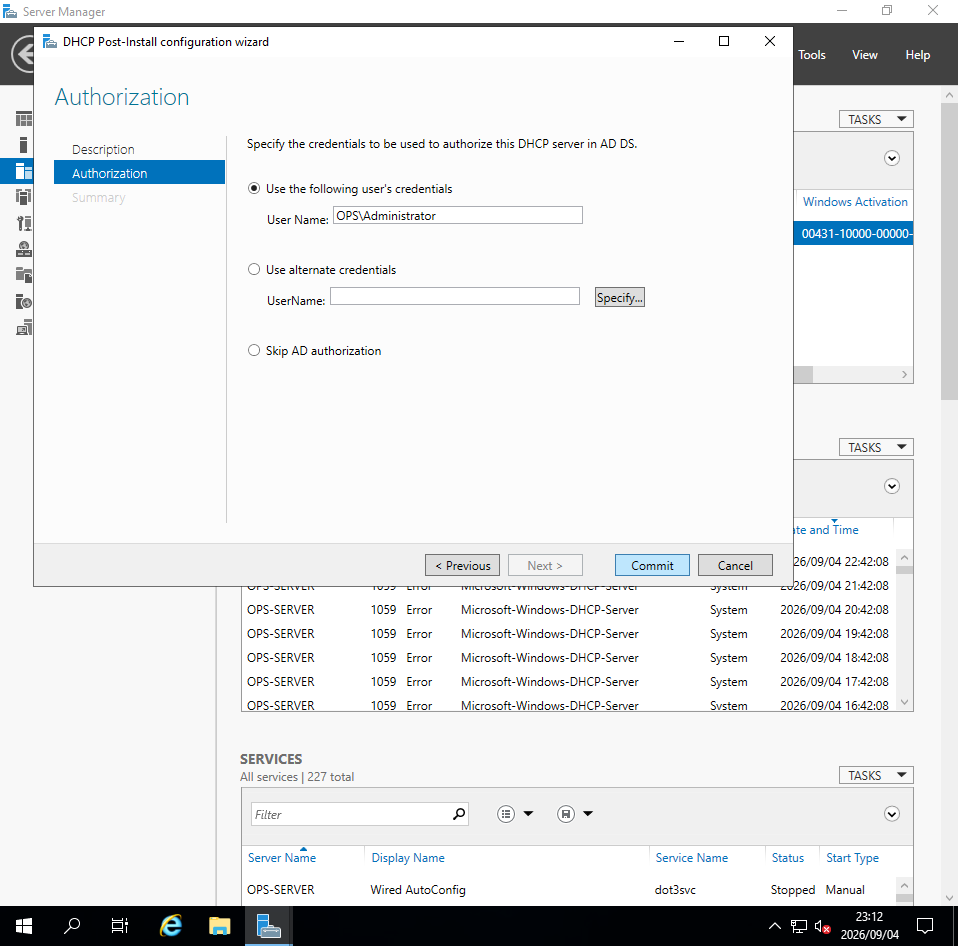
\includegraphics[width=0.7\linewidth]{Images/DHCP/DHCP_02.png}
    \caption{Authorization of DHCP Post-Install Configuration Wizard}
\end{figure}

\begin{figure}[H]
    \centering
    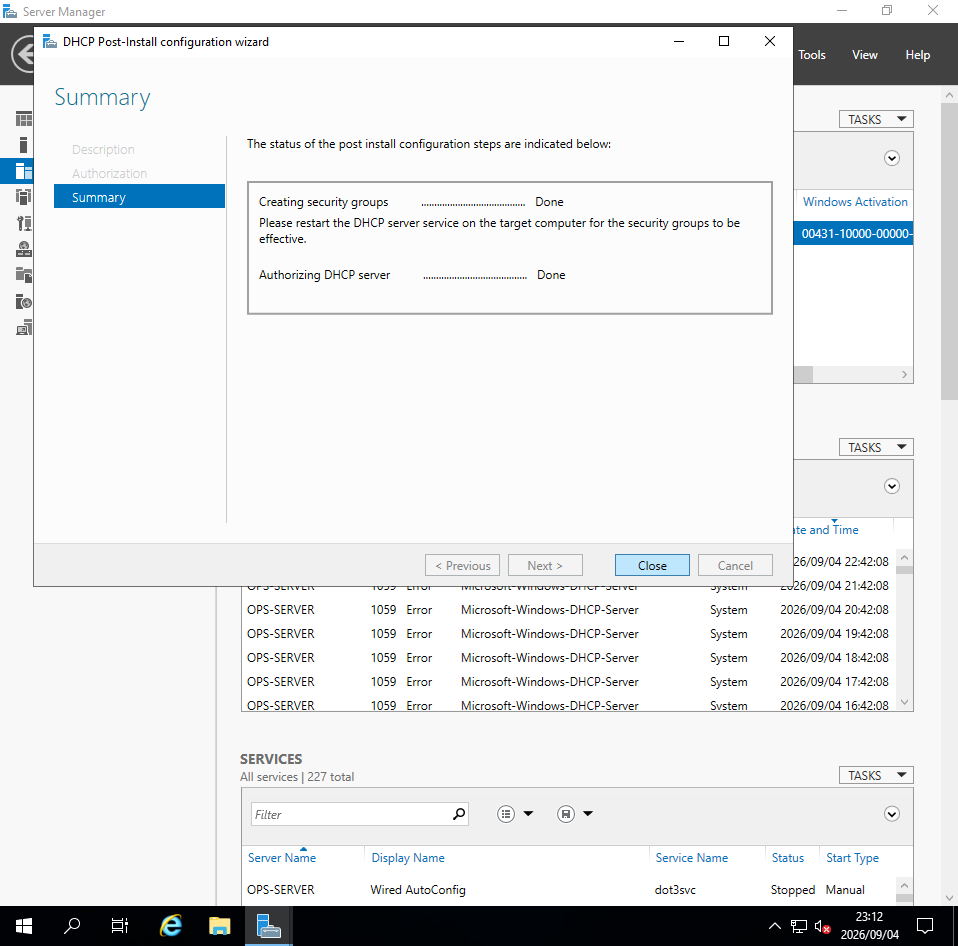
\includegraphics[width=0.7\linewidth]{Images/DHCP/DHCP_03.png}
    \caption{Post Install Configuration Completed}
\end{figure}

\subsection{The DHCP Scope}
\paragraph{}
For a DHCP server to hand out IP addresses, it needs to know IP addresses,
subnet mask, default gateway and DNS server addresses are within the network so that it can 
package and hand out the information to computers who request it. This package of information 
is called a DHCP scope (\cite{masterWS19}).

\paragraph{}
To begin defining the scope, we decided to launch a management tool using the Tools menu 
inside the Server Manager. This will open up a window for DHCP with the name of the device 
that the server is located on.

\begin{figure}[H]
    \centering
    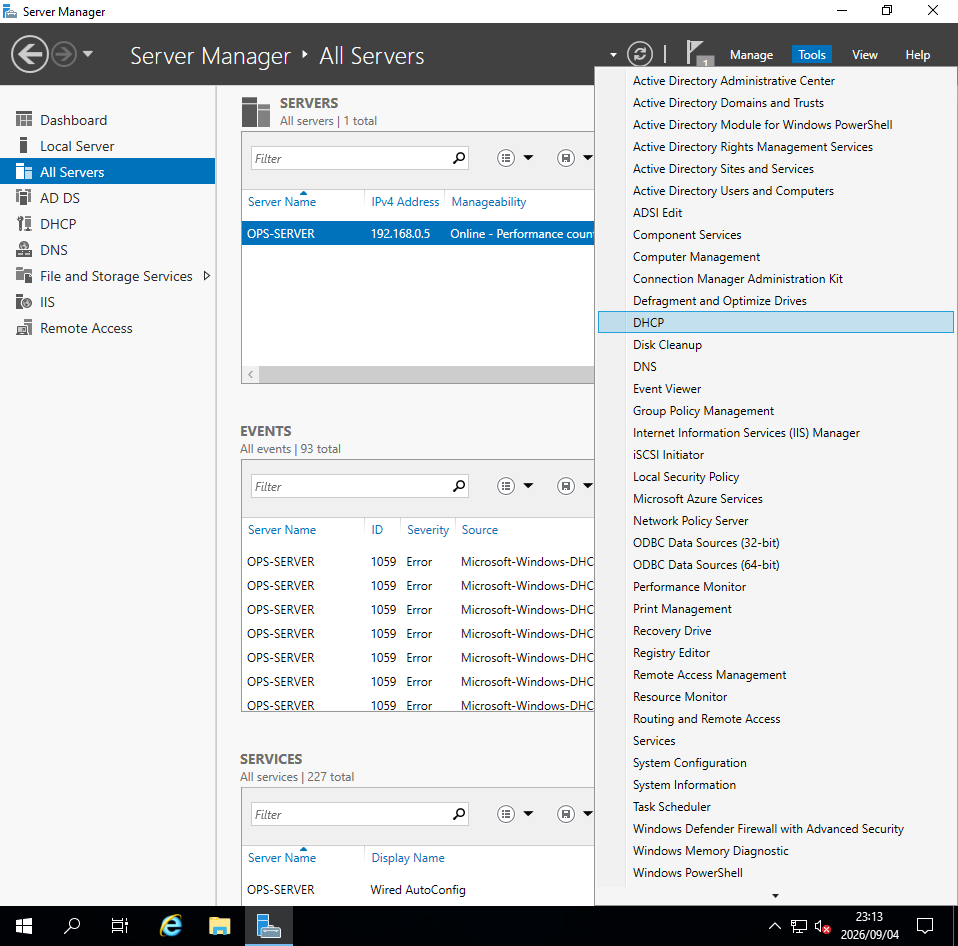
\includegraphics[width=0.7\linewidth]{Images/DHCP/DHCP_04.png}\
    \caption{DHCP Selected on Tools Dropdown Menu}
\end{figure}

\begin{figure}[H]
    \centering
    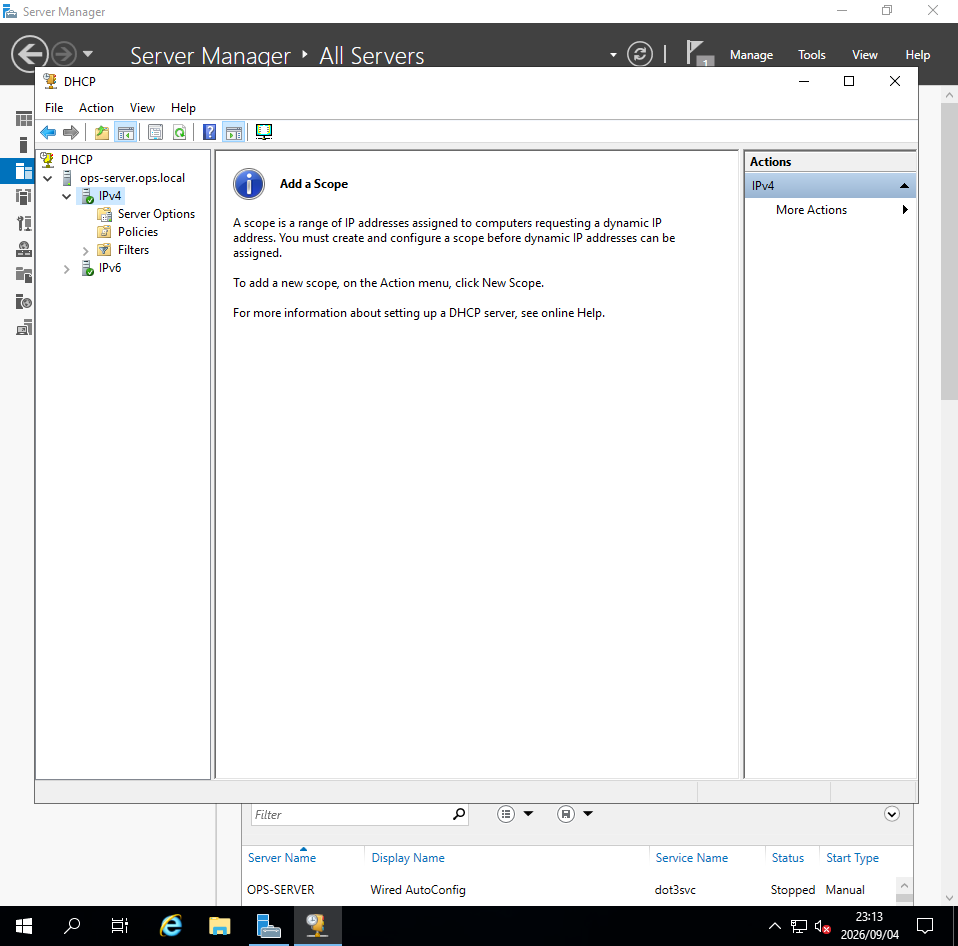
\includegraphics[width=0.7\linewidth]{Images/DHCP/DHCP_05.png}
    \caption{DHCP Windows}
\end{figure}
%two figures

\paragraph{}
After opening the DHCP window, the computer was selected and dropped down two protocols: IPv4 and IPv6.
The former was selected and first left-clicked on, where it gave information regarding the addition of a scope, along with the server 
options, policies and filters. This protocol did not have a scope as yet, so it needed to be configured.
To properly begin the process, IPv4 was right-clicked on, giving a drop-down menu when the option to add 
a new scope was present. Choosing this option opened the New Scope Wizard. After clicking next on the wizard, the basics 
of the scope needed to be decided. The name given was GROUP 1-SCOPE.

\begin{figure}[H]
    \centering
    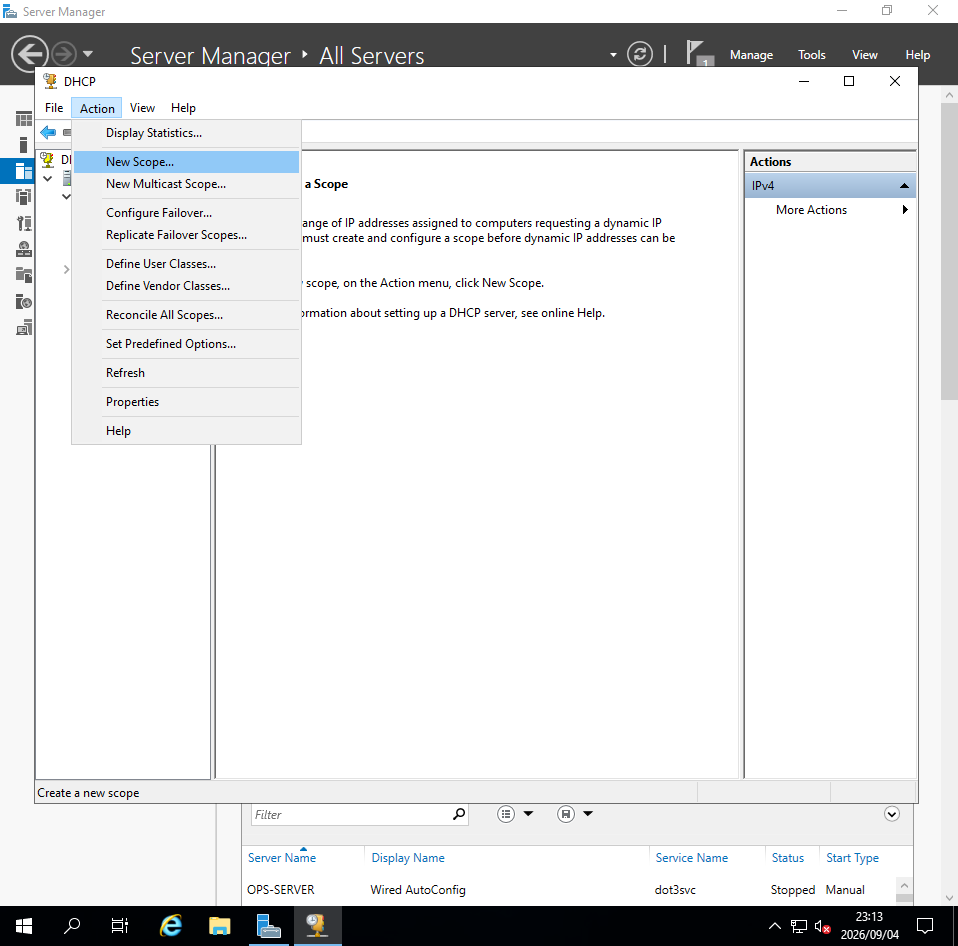
\includegraphics[width=0.7\linewidth]{Images/DHCP/DHCP_06.png}
    \caption{Adding a Scope}
\end{figure}
\begin{figure}[H]
    \centering
    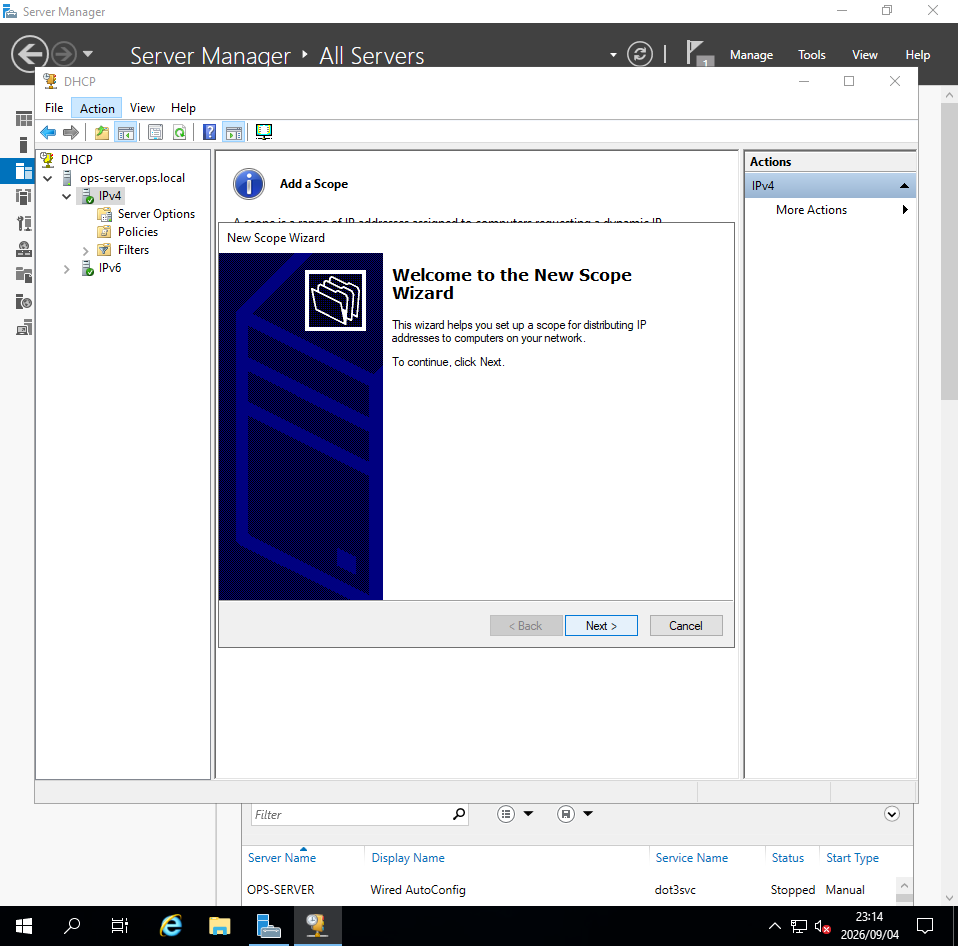
\includegraphics[width=0.7\linewidth]{Images/DHCP/DHCP_07.png}
    \caption{New Scope Wizard}
\end{figure}

\begin{figure}[H]
    \centering
    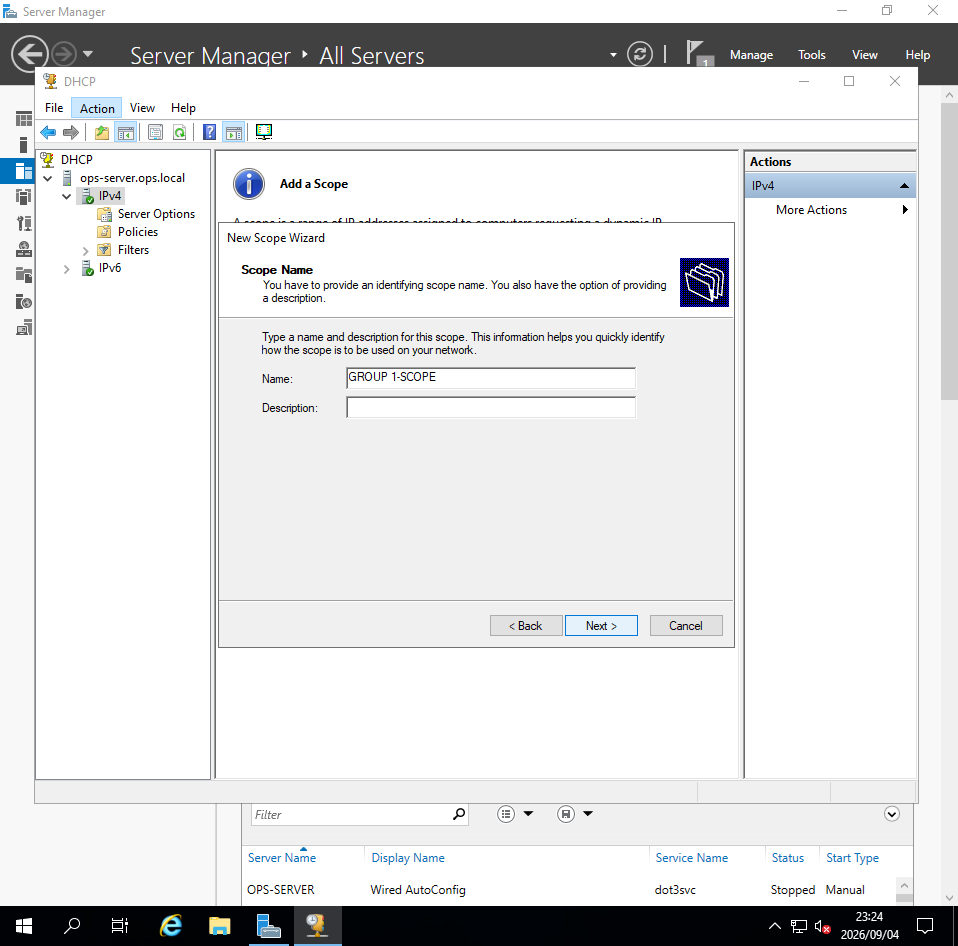
\includegraphics[width=0.7\linewidth]{Images/DHCP/DHCP_08.png}
    \caption{Group One Scope Made}
\end{figure}

\paragraph{}
There exists 4.3 billion posible IPv4 addresses and 3.7 billion available addresses, and therefore,
there exists a countless amount of possible addresses that the scope can allow (\cite{ffIP}).
A scope does not need to accomodate billions of addresses, it just needs a few hundred or a few dozen.
When configuring it, the range of IP addresses needed to be decided.
The addresses that the scope will hand out were from 
192.168.0.100 to 192.168.0.254. This will be the address pool. There were no exclusions 
or delays made in the scope. Alongside handed out IPs, the scope also has
the option to configure the amount of time that a client keeps an assigned IP before renewal, ensuring 
efficient management of IP addresses (\cite{rapidseedbox}). This period of
time is called the lease duration. It was left at the default number of 8 days.

\begin{figure}[H]
    \centering
    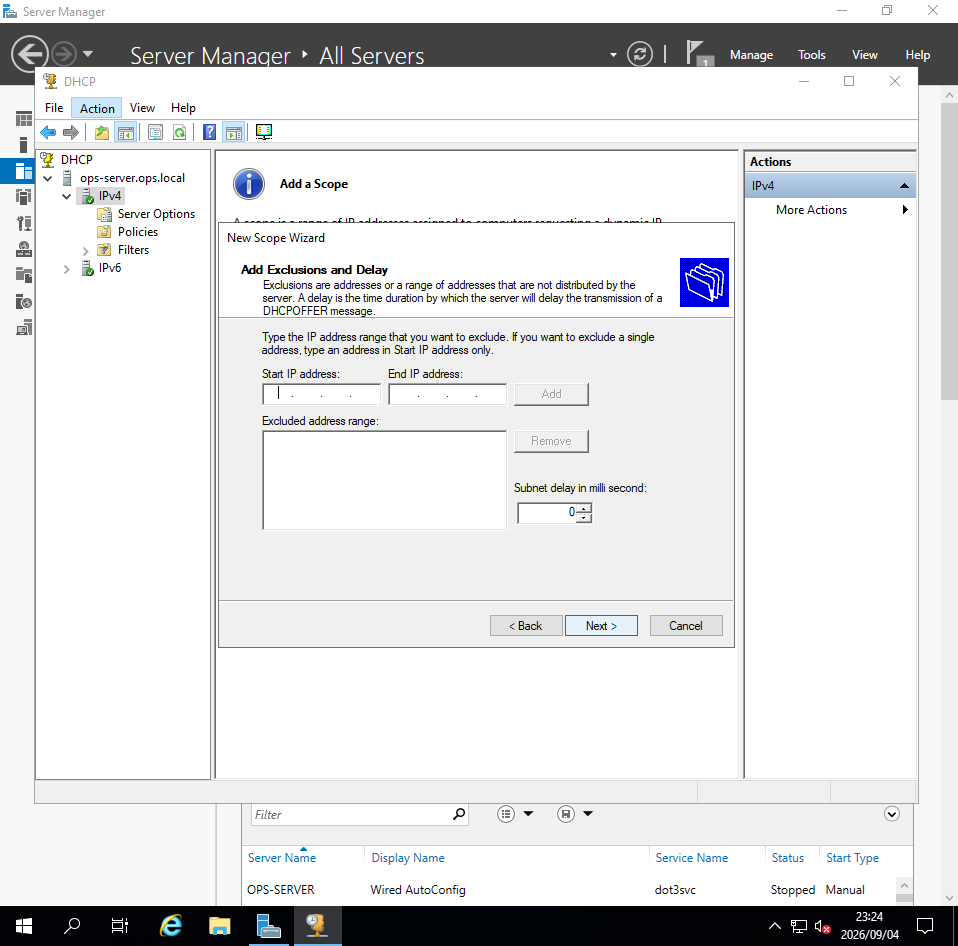
\includegraphics[width=0.7\linewidth]{Images/DHCP/DHCP_10.png}
    \caption{No Exclusions made}
\end{figure}

\begin{figure}[H]
    \centering
    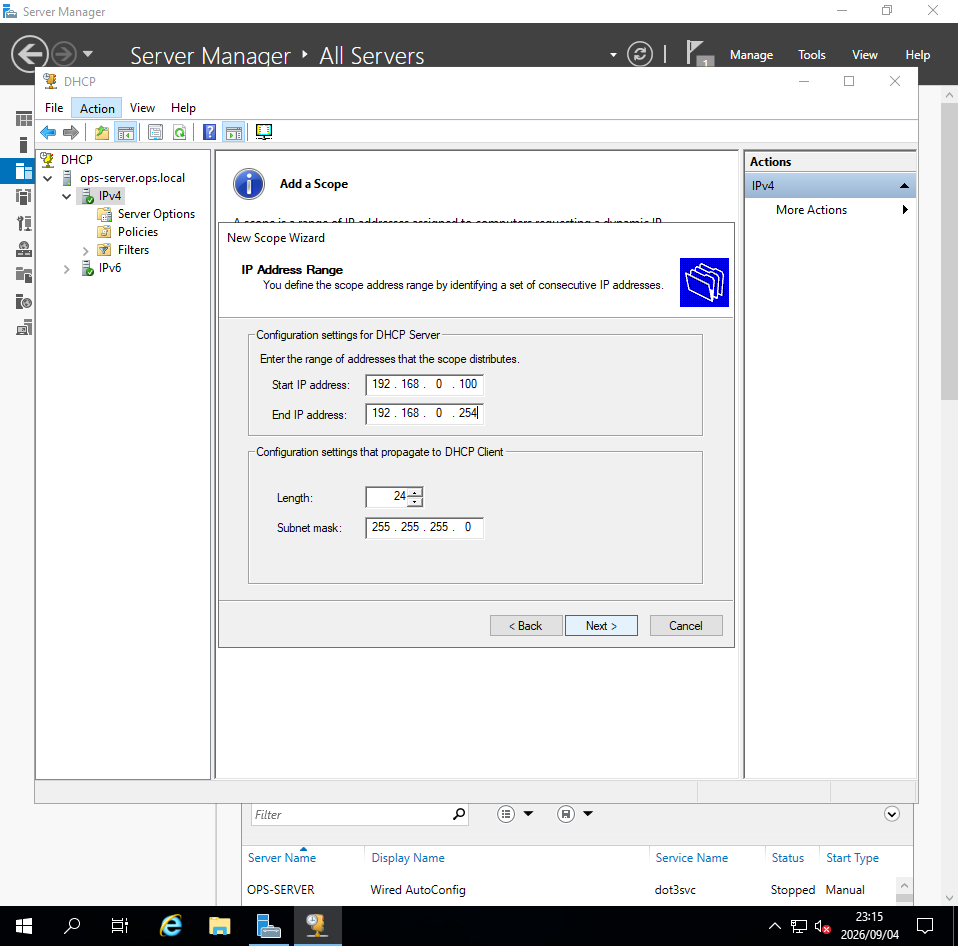
\includegraphics[width=0.7\linewidth]{Images/DHCP/DHCP_09.png}
    \caption{Setting IP Address Range}
\end{figure}

\begin{figure}[H]
    \centering
    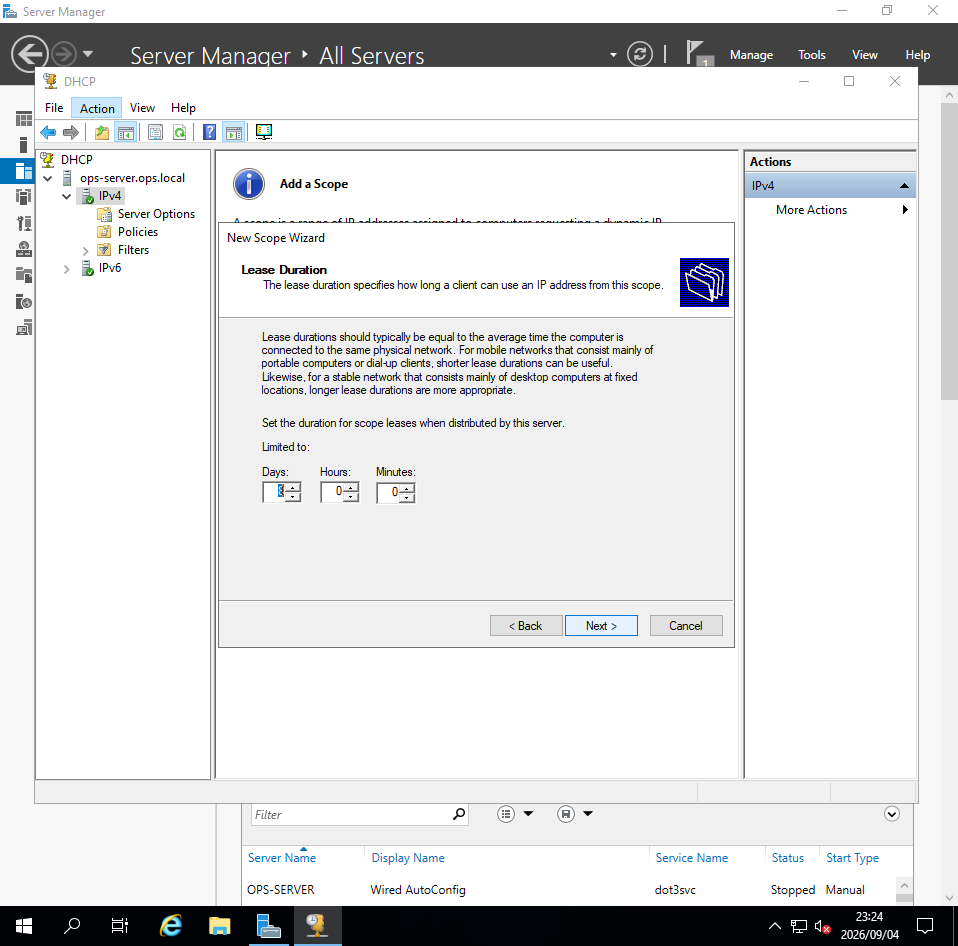
\includegraphics[width=0.7\linewidth]{Images/DHCP/DHCP_11.png}
    \caption{Lease duration of 8 days set}
\end{figure}

\paragraph{}
When clients use the server, access to the internet is an important 
feature that must be present in the server. 
In order for the clients to able to access the internet, 
they need to be able to talk to other devices and networks outside of the DHCP subnet.
A default gateway allows for this. Without it, a client can only reach devices and networks inside 
its own subnet. The default gateway was given the IP address of 192.168.0.1.

\begin{figure}[H]
    \centering
    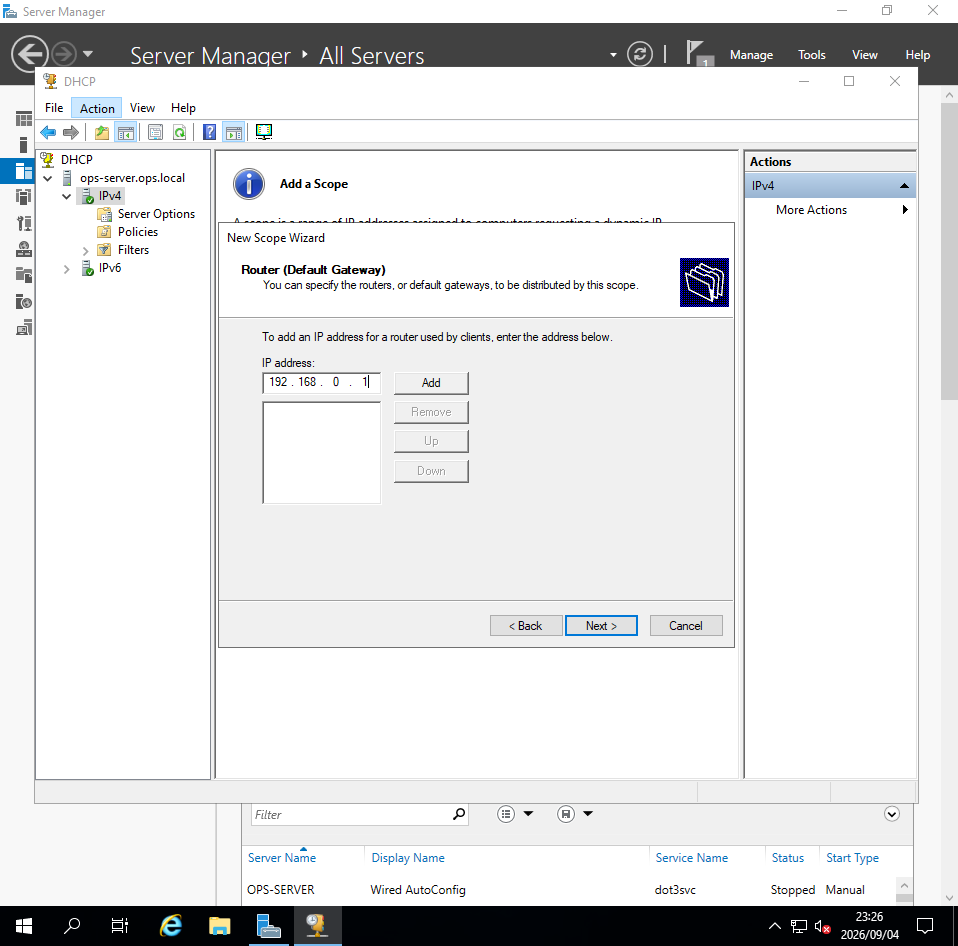
\includegraphics[width=0.7\linewidth]{Images/DHCP/DHCP_12.png}
    \caption{Default Gateway Configured (1)}
\end{figure}

\begin{figure}[H]
    \centering
    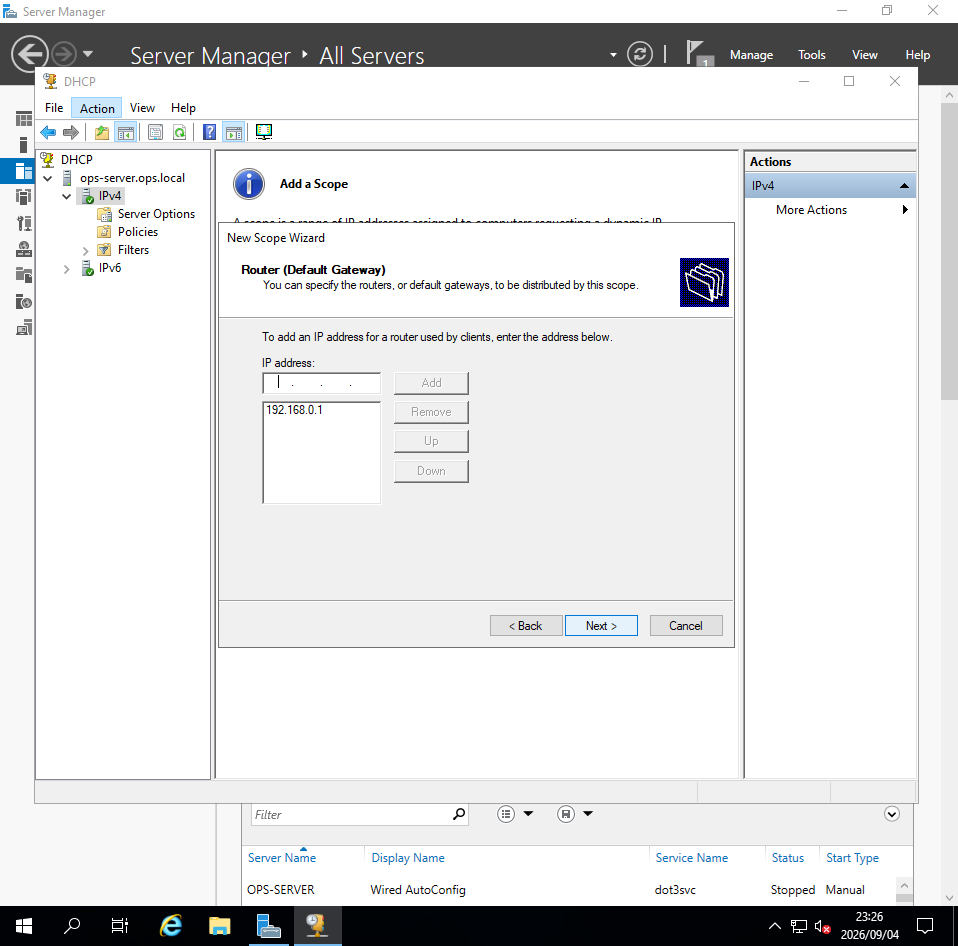
\includegraphics[width=0.7\linewidth]{Images/DHCP/DHCP_13.png}
    \caption{Default Gateway Configured (2)}
\end{figure}

\paragraph{}
After the setting up of the default gateway, the next step was setting up the DNS server.
As mentioned earlier, the DHCP has the job of handing out IP addresses and more for a client to be 
able to use the network. An IP allows a device to communicate with other hosts, but IP addresses 
are inconvinient to memorize or type down. The DNS Server and Domain Name exist 
to allow for devices to access the DHCP server through use of IPs that resolve into domain names (\cite{dns}).
The domain name was set to OPS.local and two IPs, 192.168.0.5 and 8.8.8.8, for two servers were set.
This would mean that in order to access the server they would simply need to type in the domain name, making it 
more accessible for non-domain joined machines.

\begin{figure}[H]
    \centering
    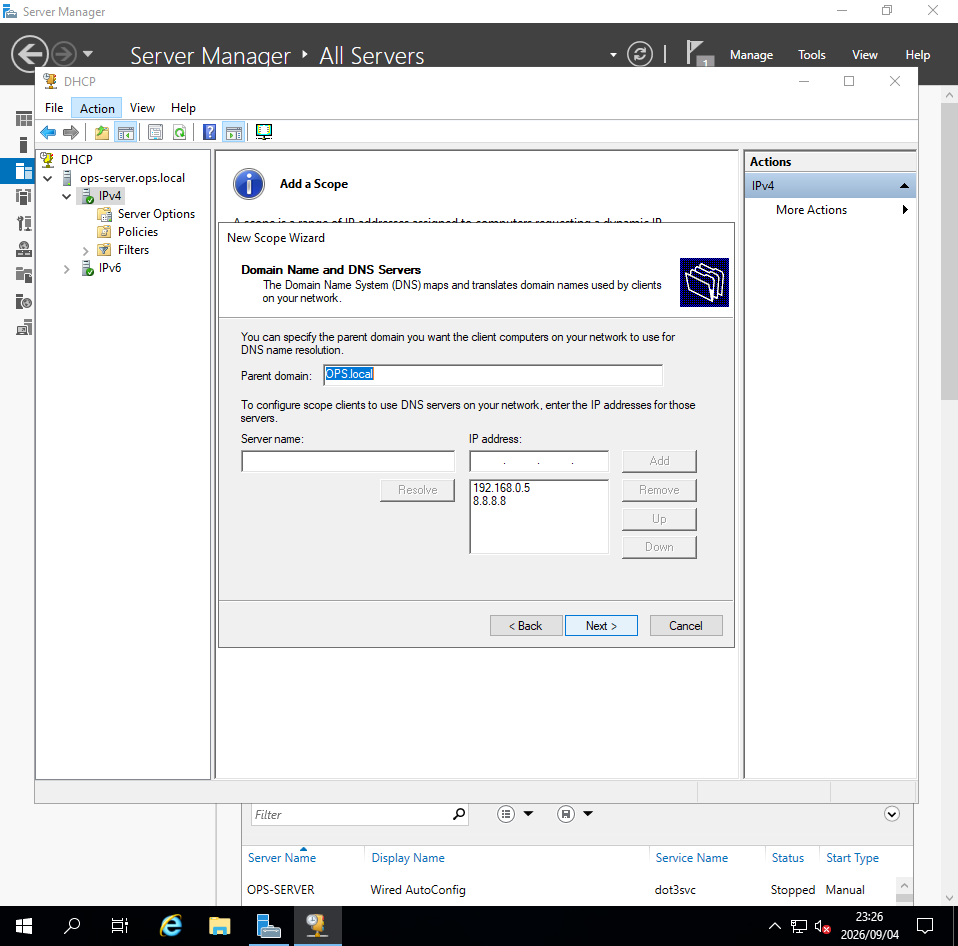
\includegraphics[width=0.7\linewidth]{Images/DHCP/DHCP_14.png}
    \caption{DNS Server and Domain Name}
\end{figure}

\paragraph{}
After the DNS Server and Domain Names are configured, 
there was an option for WINS Server configuration. WINS is a part of the scope 
that resolves NetBOIS computer names to IP Addresses. It is needed to support pre-Windows 2000 
systems and older application using NetBOIS over TCP/IP (\cite{wins}). None of the systems planned to be connected in the network 
do not qualify as pre-Windows 2000 systems, there WINS is not needed.

\begin{figure}[H]
    \centering
    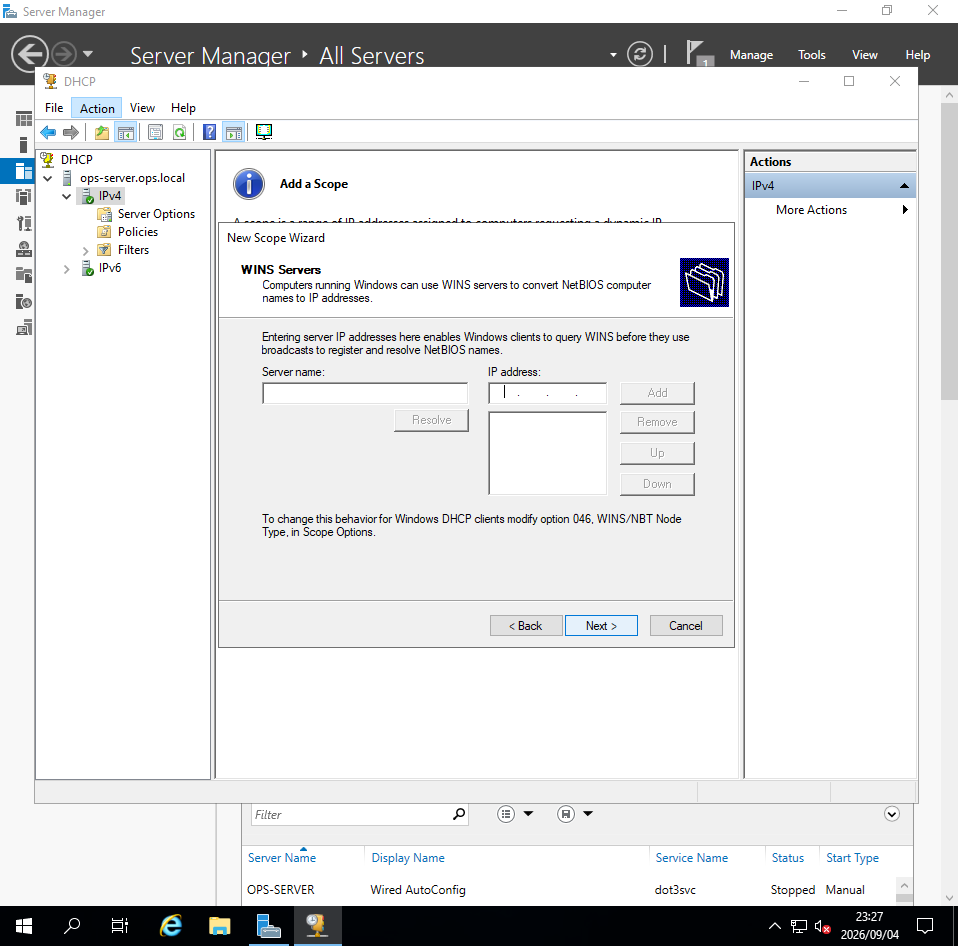
\includegraphics[width=0.7\linewidth]{Images/DHCP/DHCP_15.png}
    \caption{WINS Server configurinf left vacant}
\end{figure}

\paragraph{}
All necessary parts of the scope have been configured. After passing the WINS Server configuring, all that was left was activation of the scope.
Upon activating the scope, the wizard will present completion display. To close the wizard, the finish button was clicked. 
The scope is now activated and ready for testing. The scope will now had out IP addresses from 
192.168.0.100 to 192.168.0.254 and this will be its address pool. At the time of the creation of the scope, 
there were no address leases yet.

\begin{figure}[H]
    \centering
    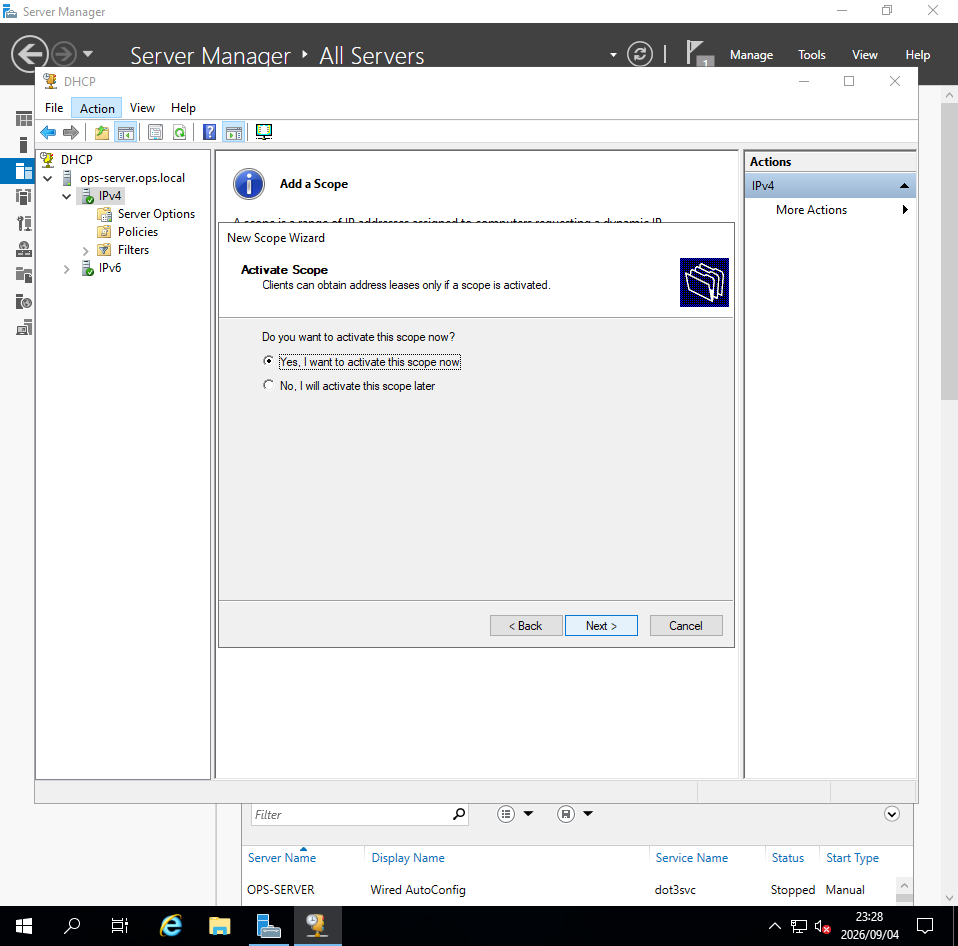
\includegraphics[width=0.7\linewidth]{Images/DHCP/DHCP_16.png}
    \caption{Activation of Scope}
\end{figure}

\begin{figure}[H]
    \centering
    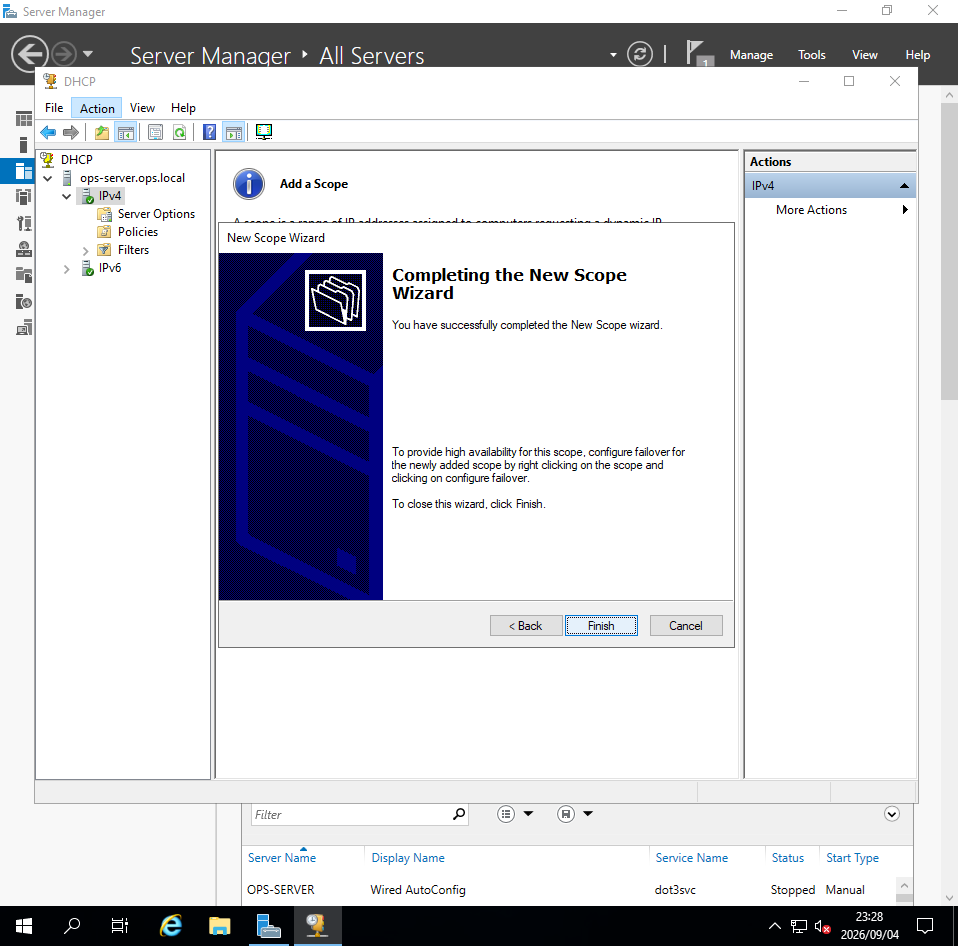
\includegraphics[width=0.7\linewidth]{Images/DHCP/DHCP_17.png}
    \caption{Finishing New Scope Wizard}
\end{figure}
\begin{figure}[H]
    \centering
    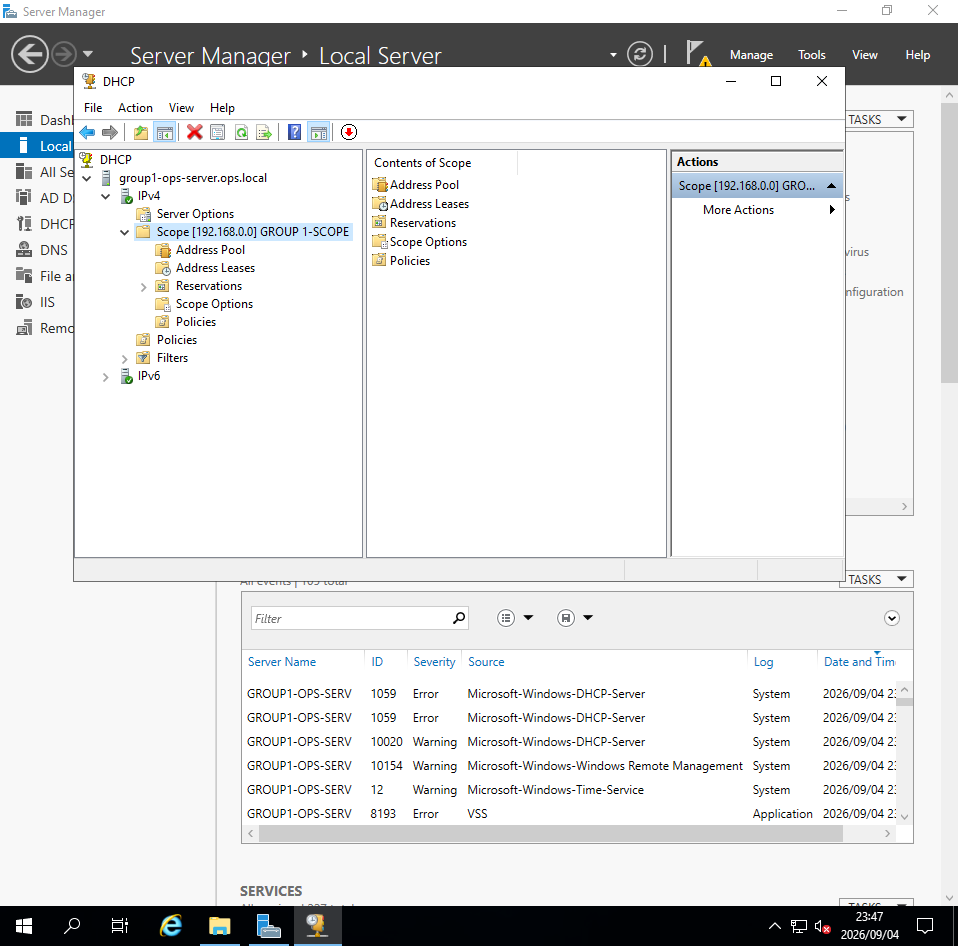
\includegraphics[width=0.7\linewidth]{Images/DHCP/DHCP_18.png}
    \caption{New DHCP Scope created}
\end{figure}

\subsection{Testing of DHCP Server}

